\documentclass[tikz,border=10pt]{standalone}
\usepackage{tikz}
\usepackage{xcolor}
\usetikzlibrary{shapes,arrows,positioning,fit,backgrounds}

% Define colors
\definecolor{inputcolor}{RGB}{225,245,254}
\definecolor{processcolor}{RGB}{243,229,245}
\definecolor{featurecolor}{RGB}{232,245,232}
\definecolor{fusioncolor}{RGB}{255,243,224}
\definecolor{ensemblecolor}{RGB}{252,228,236}
\definecolor{privacycolor}{RGB}{187,222,251}
\definecolor{outputcolor}{RGB}{255,235,238}

\begin{document}

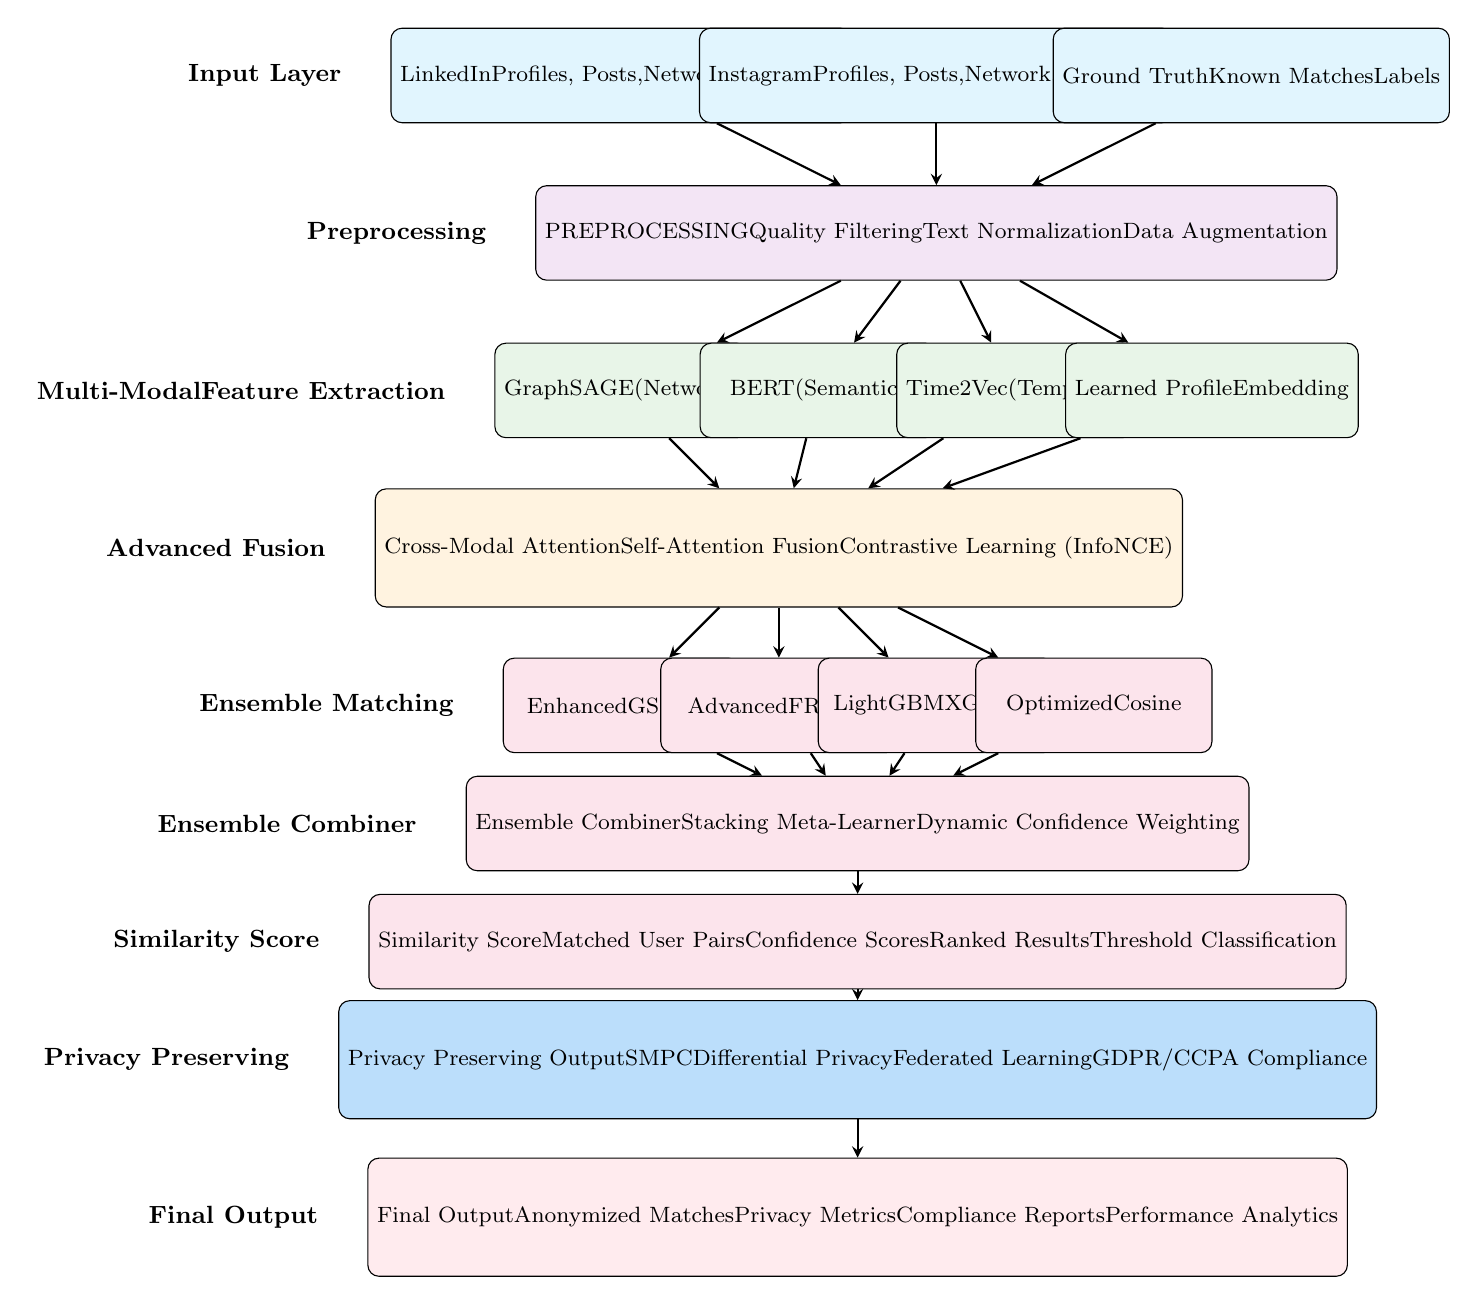
\begin{tikzpicture}[
    node distance=1.5cm,
    box/.style={rectangle, rounded corners, minimum width=3cm, minimum height=1.2cm, text centered, draw=black, fill=white, font=\footnotesize},
    inputbox/.style={box, fill=inputcolor},
    processbox/.style={box, fill=processcolor},
    featurebox/.style={box, fill=featurecolor},
    fusionbox/.style={box, fill=fusioncolor},
    ensemblebox/.style={box, fill=ensemblecolor},
    privacybox/.style={box, fill=privacycolor},
    outputbox/.style={box, fill=outputcolor},
    arrow/.style={thick,->,>=stealth},
    wide/.style={minimum width=4cm},
    tall/.style={minimum height=1.5cm}
]

% Input Layer
\node[inputbox, wide] (linkedin) at (0,12) {LinkedIn\\Profiles, Posts,\\Network, Metadata};
\node[inputbox, wide] (instagram) at (4,12) {Instagram\\Profiles, Posts,\\Network, Metadata};
\node[inputbox, wide] (groundtruth) at (8,12) {Ground Truth\\Known Matches\\Labels};

% Preprocessing
\node[processbox, wide] (preprocessing) at (4,10) {PREPROCESSING\\Quality Filtering\\Text Normalization\\Data Augmentation};

% Multi-Modal Feature Extraction
\node[featurebox] (graphsage) at (0,8) {GraphSAGE\\(Network)};
\node[featurebox] (bert) at (2.5,8) {BERT\\(Semantic)};
\node[featurebox] (time2vec) at (5,8) {Time2Vec\\(Temporal)};
\node[featurebox] (profile) at (7.5,8) {Learned Profile\\Embedding};

% Advanced Fusion
\node[fusionbox, wide, tall] (crossmodal) at (2,6) {Cross-Modal Attention\\Self-Attention Fusion\\Contrastive Learning (InfoNCE)};

% Ensemble Matching
\node[ensemblebox] (gsmua) at (0,4) {Enhanced\\GSMUA};
\node[ensemblebox] (fruip) at (2,4) {Advanced\\FRUI-P};
\node[ensemblebox] (lightgbm) at (4,4) {LightGBM\\XGBoost};
\node[ensemblebox] (cosine) at (6,4) {Optimized\\Cosine};

% Ensemble Combiner
\node[ensemblebox, wide] (combiner) at (3,2.5) {Ensemble Combiner\\Stacking Meta-Learner\\Dynamic Confidence Weighting};

% Similarity Score
\node[ensemblebox, wide] (similarity) at (3,1) {Similarity Score\\Matched User Pairs\\Confidence Scores\\Ranked Results\\Threshold Classification};

% Privacy Preserving Output
\node[privacybox, wide, tall] (privacy) at (3,-0.5) {Privacy Preserving Output\\SMPC\\Differential Privacy\\Federated Learning\\GDPR/CCPA Compliance};

% Final Output
\node[outputbox, wide, tall] (finaloutput) at (3,-2.5) {Final Output\\Anonymized Matches\\Privacy Metrics\\Compliance Reports\\Performance Analytics};

% Arrows
\draw[arrow] (linkedin) -- (preprocessing);
\draw[arrow] (instagram) -- (preprocessing);
\draw[arrow] (groundtruth) -- (preprocessing);

\draw[arrow] (preprocessing) -- (graphsage);
\draw[arrow] (preprocessing) -- (bert);
\draw[arrow] (preprocessing) -- (time2vec);
\draw[arrow] (preprocessing) -- (profile);

\draw[arrow] (graphsage) -- (crossmodal);
\draw[arrow] (bert) -- (crossmodal);
\draw[arrow] (time2vec) -- (crossmodal);
\draw[arrow] (profile) -- (crossmodal);

\draw[arrow] (crossmodal) -- (gsmua);
\draw[arrow] (crossmodal) -- (fruip);
\draw[arrow] (crossmodal) -- (lightgbm);
\draw[arrow] (crossmodal) -- (cosine);

\draw[arrow] (gsmua) -- (combiner);
\draw[arrow] (fruip) -- (combiner);
\draw[arrow] (lightgbm) -- (combiner);
\draw[arrow] (cosine) -- (combiner);

\draw[arrow] (combiner) -- (similarity);
\draw[arrow] (similarity) -- (privacy);
\draw[arrow] (privacy) -- (finaloutput);

% Layer labels
\node[left=0.5cm of linkedin, font=\small\bfseries] {Input Layer};
\node[left=0.5cm of preprocessing, font=\small\bfseries] {Preprocessing};
\node[left=0.5cm of graphsage, font=\small\bfseries] {Multi-Modal\\Feature Extraction};
\node[left=0.5cm of crossmodal, font=\small\bfseries] {Advanced Fusion};
\node[left=0.5cm of gsmua, font=\small\bfseries] {Ensemble Matching};
\node[left=0.5cm of combiner, font=\small\bfseries] {Ensemble Combiner};
\node[left=0.5cm of similarity, font=\small\bfseries] {Similarity Score};
\node[left=0.5cm of privacy, font=\small\bfseries] {Privacy Preserving};
\node[left=0.5cm of finaloutput, font=\small\bfseries] {Final Output};

\end{tikzpicture}

\end{document}
